\documentclass[hyperref={pdfpagelabels=false}]{beamer}
\usepackage{lmodern}
\usepackage[demo]{graphicx}
% \usepackage{caption}
% \usepackage{subcaption}
\usetheme{Frankfurt}
\usecolortheme{crane}

\title{Mysteries of Mysterion}  
\author{\texttt{CrypTrio}} 
\institute{
	
\includegraphics[scale=0.08]{logoiitbh}
	
	Department of \texttt{<Computer Science>}\\ 
	Indian Institute of Technology Bhilai}

\begin{document}
	\begin{frame}
	\titlepage

\end{frame} 

\AtBeginSection[]
{
	\begin{frame}<beamer>
	\frametitle{Outline}
	\tableofcontents[currentsection]
\end{frame}
}

\section{Introduction}

\begin{frame}{Introduction}
\begin{itemize}
    \item Block Cipher 
    \item XLS design 
    % (similar to SPN)
    \item It's security margins is similar with AES cipher 
    \item It has 4-bit S-boxes and 32-bit L-boxes and Shift Columns operation.
\end{itemize}
\end{frame}

\begin{frame}{Bit-Slicing}
    \begin{itemize}
        \item Converting the cipher into bit-wise operations (like the way we'd implement it in hardware)
        \item Carrying out those bit wise operations in parallel
    \end{itemize}
\end{frame}

\begin{frame}{XLS-Design}
\begin{itemize}
    \item LS Designs are a combination of linear diffusion L-boxes and non-linear bitslice S-boxes.
    \item These are  susceptible to invariant subspace attacks.
    \item So, XLS (eXtended LS) Designs model is developed by adding the Shiftcolumns operation to LS design models
    \item XLS-design comprises of SuperS-boxes, made of optimal components - 4-bit S-boxes and 32-bit L-boxes, and ShiftColumns operation.
\end{itemize}
\end{frame}

\begin{frame}{LS Design Model}


% \begin{figure}[H]
%      \centering
%     \subfloat[ls]{{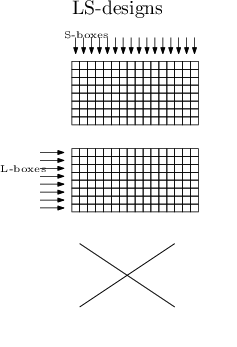
\includegraphics[width=4cm]{ls.png} }}%
%     % \qquad
%     % \subfloat[xls]{{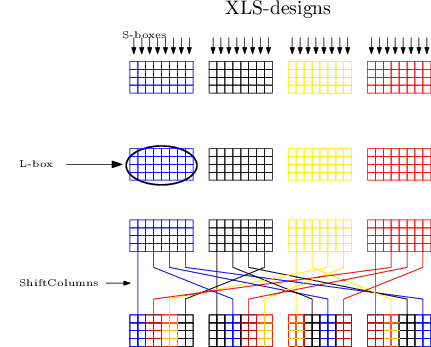
\includegraphics[width=4cm]{xls.png} }}%
    
%     \end{figure}
\begin{center}
    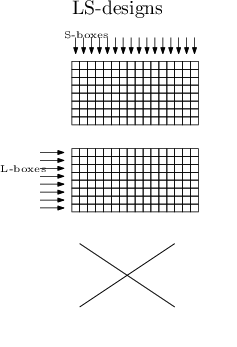
\includegraphics[width=4cm]{ls.png}
\end{center}

\end{frame}

\begin{frame}{XLS Design Model}
\begin{center}
    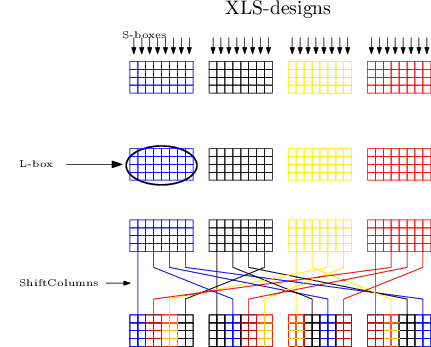
\includegraphics[width=5cm]{xls.png}
\end{center}
\end{frame}

\section{Cipher Specifications}

\begin{frame}{S-box}

\begin{itemize}
    \item Mysterion uses S-boxes that has bitslice representation with a combination of AND (also OR) and XOR gates. 
    \item It has a bitslice representation of 4 AND (precisely 3 AND and 1 OR) gates and 4 XOR gates
    \item It has a  differential probability of $2^{-2}$ and linear probability $2^{-1}$
\end{itemize}
\end{frame}

\begin{frame}{DDT \& LAT}
    \begin{figure}
    \centering
    \begin{subfigure}{}
      \centering
      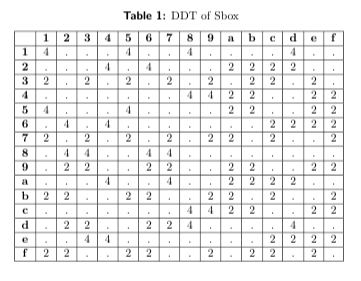
\includegraphics[scale=0.37]{DDT.png}
      \label{fig:sub1}
    \end{subfigure}%
    \begin{subfigure}{}
      \centering
      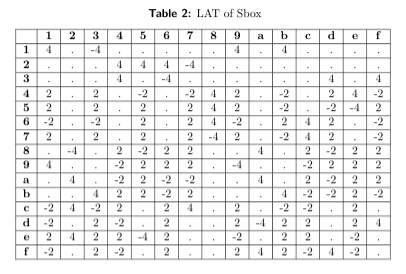
\includegraphics[scale=0.38]{LAT.png}
      \label{fig:sub2}
    \end{subfigure}
    \label{fig:test}
    \end{figure}
    \begin{block} {Observations}
    Differential probability = $\dfrac{4}{16}$ = $2^{-2}$ \\
    Linear probability = $\dfrac{4}{8}$ = $2^{-1}$ 
    \end{block}
\end{frame}

\begin{frame}{L-box}

    \begin{itemize}
        \item Its purpose is to diffuse changes in the state.
        \item linear transformation
        \item The algorithm which finds recursive MDS diffusion layers using shortened BCH codes from paper []
        \item When this is run using Magma code paper [] with $k =8$ and $s = 4$ as input gives polynomials whose companion matrix $C_m$ raised to power $8$ $\implies C^8_m$ gives us the MDS matrix 
     \end{itemize}
\end{frame}
\begin{frame}{Shift Columns}

    \begin{itemize}
        \item In Mysterion-128, as there are 4 blocks (with each block having 8 columns) ShiftColumns acts on columns two by two.
        \item In Mysterion-256 as there are 8 blocks (with each block having 8 columns) ShiftColumns acts on columns one by one
    \end{itemize}
\end{frame}

\begin{frame}{Diagrams}


\begin{center}
\begin{figure}[h!]
  \caption{Shift Columns-128}
   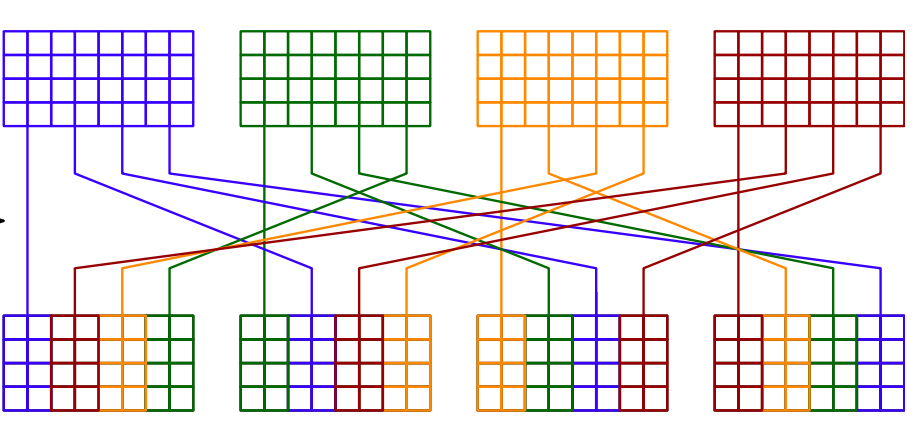
\includegraphics[width=6cm\textwidth]{128.png} 
\end{figure}
   
\end{center}

\begin{center}
\begin{figure}[h!]
  \caption{Shift Columns-256}
   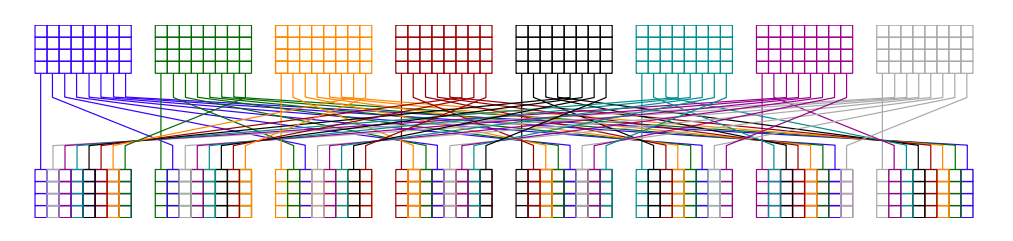
\includegraphics[width=10cm\textwidth]{256.png} 
\end{figure}
\end{center}

\end{frame}

\begin{frame}{Round constant and Key}
    \begin{itemize}
        \item Up until now, we have done nothing to make the ciphertext dependent on the key. So to do this, we add the key to the state. 
        \item The Mysterion block cipher has no key schedule. In every round, the same key is added to the state.
    \end{itemize}
\end{frame}
\section{Security Analysis}

\begin{frame}{Boomerang Attack}
\begin{itemize}
    \item Special Differential Cryptanalysis
    \item two differentials for the two sub ciphers $C_0$ and $C_1$ obtained from cipher $C$ 
    \item $C=C_{0} \circ C_{1}$
    \item shorter differentials have more better probabilities $\implies$ improved results 
\end{itemize}
\begin{block}{Theorems}
\textbf{Theorem 1:}  Four rounds of Mysterion-128 has at least 45 active S-boxes.  \\
\textbf{Theorem 2:} Four rounds of Mysterion-256 has at least 81 active S-boxes. \\
\end{block}

\end{frame}

\begin{frame}{Boomerang Attack}
\begin{enumerate}
    \item For 128 bit : \\
    We use the Theorem 1  to find the max differential prob that can be obtained : 
    $$\text{Pr}_{diff}(4R) \leq \text{Pr}_{diff}^{max}(Sbox)^{45} = (2^{-2})^{45} = 2^{-90} $$
    $$\implies \text{Pr}_{diff}^{max}(8R) = \text{Pr}_{diff}(4R) *\text{Pr}_{diff}(4R)  = 2^{-90}*2^{-90} = 2^{-180}  
    $$
    the Pr obtained is way less that  brute force probability ($2^{-128}$). \\
    
\end{enumerate}
\end{frame}

\begin{frame}{Boomerang Attack}
    \begin{enumerate}
        \item For 256 bit: \\
    We use the Theorem 2  to find the max differential prob that can be obtained : 
    $$\text{Pr}_{diff}^{max}(8R) = \text{Pr}_{diff}(4R) *\text{Pr}_{diff}(4R)  = 2^{-81*2}*2^{-81*2} = 2^{-324} 
    % >> 2^{-256} 
    $$
    the Pr obtained is way less that  brute force probability ($2^{-256}$). \\
    \end{enumerate}
\end{frame}

\begin{frame}{Integral Attack}

    \begin{itemize}
        \item Integral attacks tries to extract information about the key by observing the sum of ciphertext values.
        \item We may find integral property upto 4 rounds, and then we can mount this attack from 7-9 rounds depending on the key size. 
        \item Sufficient security margin for the full cipher, since there are 12 and 16 rounds for Mysterion -128 and Mysterion-256.
    \end{itemize}
\\\\
\textbf{Division Property - EUROCRYPT 2015}
It allows to construct more efficient integral distinguishers exploiting the limited algebraic degree of reduced ciphers.

\end{frame}

\begin{frame}{Invariant subspace Attack}
\begin{itemize}
    \item LS Design models are vulnerable to this attack 
    \item This was identified by performing an exhaustive analysis on a 32 bit block
    \item Addition of Shiftcolumns operation to LS design models (which are called as XLS models) ,this attack can no longer be done 
    \item Shiftcolumns operation prevents the propagation of subspace found for the L-box with high probability
\end{itemize}

\end{frame}

\section{Brownie Point Nominations}

\begin{frame}{ Juypter Notebook \& Online tool}
\begin{enumerate}
    \item Juypter Notebook
    \begin{enumerate}
        \item Fully interactive
        \item Complete Mysterion-128 implementation
        \item Inverse of Mysterion-128 implemented
        \item Implemented Inverse of sbox, lbox and shift columns-128 and 256 
        \item DDT and LAT analysis
        \item Example run of all functions used
    \end{enumerate}
    \item Hosted first ever Mysterion online tool at : \url{https://mysterion-tool.herokuapp.com/}
\end{enumerate}

\end{frame}

\section{Conclusion}

\begin{frame}{Simple yet Secure}
\begin{itemize}
    \item Simple heuristics
    \item Security margin for physical attacks
    \item Efficient XLS-design 
\end{itemize}
\end{frame}


\begin{frame}{Links}
    \begin{block}{}
	\begin{itemize}
		\item Implementation Source Code Link: \url{https://github.com/Meghana-12/Mysterion}
		\item Google Collab Link: \url{https://colab.research.google.com/drive/1bmUl7wT4U13XY6n8cB2sV-f5cAsr0_vV?usp=sharing}
		\item Online Tool Link: \url{ https://mysterion-tool.herokuapp.com/}
		\item Online Tool Source code: \url{https://github.com/RotonEvan/mysterious-ions}
	\end{itemize}
\end{block}
\end{frame}
% \begin{frame}{References}
% % \begin{block}{References}
% 	\begin{itemize}
% 		\item 
% 		\item  
% 		\item
% 	\end{itemize}
% % \end{block}
% \end{frame}

\begin{frame}{Thanks}
\begin{block}{Team Members}
	\begin{itemize}
		\item Gundu Shreya
		\item Varanasi Meghana
		\item Debajyoti Halder
	\end{itemize}
\end{block}
\end{frame}

\end{document}